\chapter{Sensitivity with respect to other model 
parameters (study in chapter 3)}\label{sensitivitystudy}

Here, we briefly discuss the sensitivity of our model results with
respect to variations in model parameters that have not been
investigated in detail above. To this end, we individually vary
selected parameters, leaving all other parameters at their reference
values compiled in Tab.\ \ref{input}. The target parameter for this
sensitivity study will be the BBL thickness that is the product of the
complex interplay between mixing and re-stratification processes, and
therefore provides a simple but useful proxy for overall model
performance.

\begin{figure}
  \noindent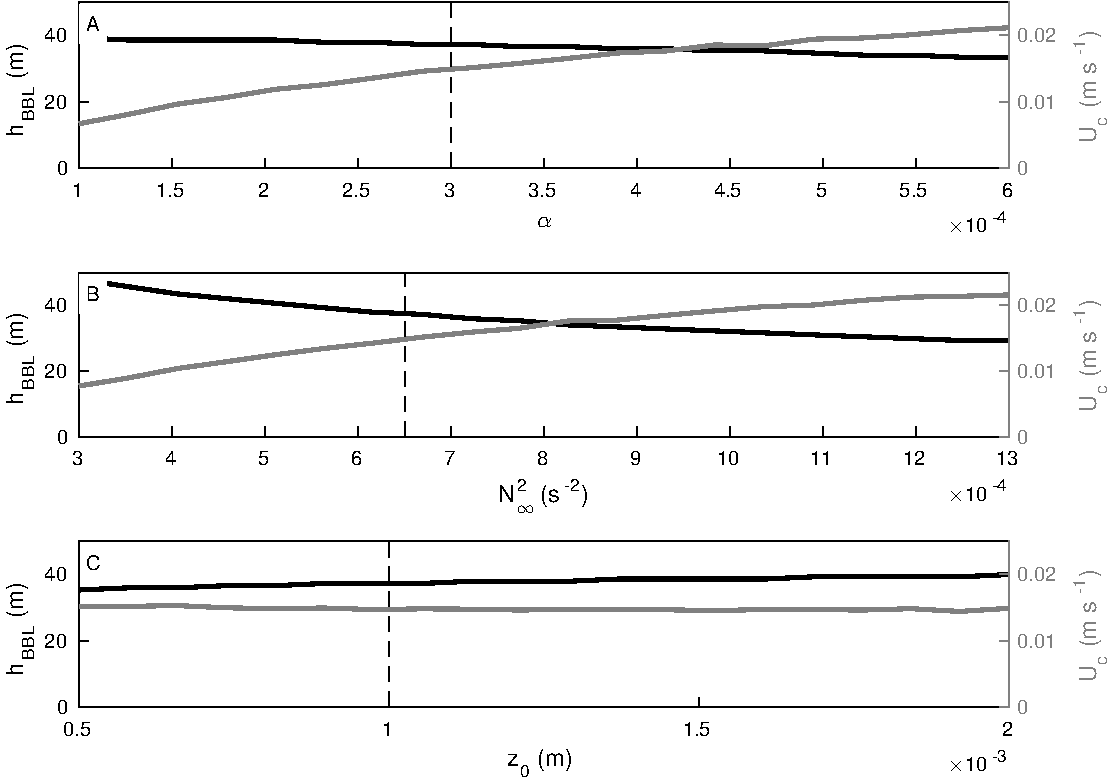
\includegraphics[width=35pc]{sensitivity.pdf}
  \caption{BBL thickness and bulk transport velocity as functions of
    (a) slope angle, (b) background stratification, and (c) bottom
    roughness. Standard parameters from Tab.\ \ref{input} are
    indicated by vertical dashed lines. }
  \label{sensitivity}
\end{figure}

Fig.\ \ref{sensitivity}a shows that a factor-2 increase or decrease of
the slope angle only results in a small (less than 10\%) change in the
computed BBL thickness. Possible uncertainties in the slope angle are
therefore of minor importance for the predicted BBL thickness. A
factor-2 increase or decrease in background stratification
(Fig.\ \ref{sensitivity}b), however, induces significant changes in
the BBL thickness, with deviations of up to 20\% from the reference
value. As our estimate of $N_\infty^2$ is based on the cross-slope
buoyancy gradient $\partial b / \partial x$ (see section
\ref{parameters}), which can be determined with good accuracy from our
high-resolution density observations at position S, we believe that
the actual uncertainty in this parameter is significantly smaller. The
least known parameter in our computations is the bottom roughness
$z_0$ that is varied in Fig.\ \ref{sensitivity}c about the reference
value $z_0 = 10^{-3}$~m. Doubling or halving $z_0$ modifies the BBL
thickness by less than 5\% with respect to the reference simulations,
with a tendency for increasing BBL thicknesses if the bottom becomes
rougher. We conclude that the uncertainties in our model parameters
are unlikely to have a large effect on the modeled BBL thickness that,
as shown above, is in good agreement with our data.


While the above parameter variations only have a small to moderate
impact on the BBL thicknesses, they do have a large influence on the
SPM fluxes, here quantified with the help of the cross-slope transport
velocity $U_c$. E.g., a 50\% decrease in the standard value for
$\alpha$ results in approximately the same reduction in the transport
velocity (Fig.\ \ref{sensitivity}a). A strong sensitivity is also
found with respect to the background stratification
(Fig.\ \ref{sensitivity}b), and only variations in the bottom
roughness show no significant effect on SPM transport
(Fig.\ \ref{sensitivity}c). Data to evaluate the significance of these
variations with respect to $U_c$ are not available.